% !TEX encoding = UTF-8 Unicode
% !TEX TS-program = xelatex

\documentclass[a4paper, 12pt]{article}
\usepackage{FDUFormat}

%\usepackage{FDUThesis}
% \usepackage{xeCJK}
\title{计时(Timing)与视觉}
\author{缪一展}
\date{}
\begin{document}
%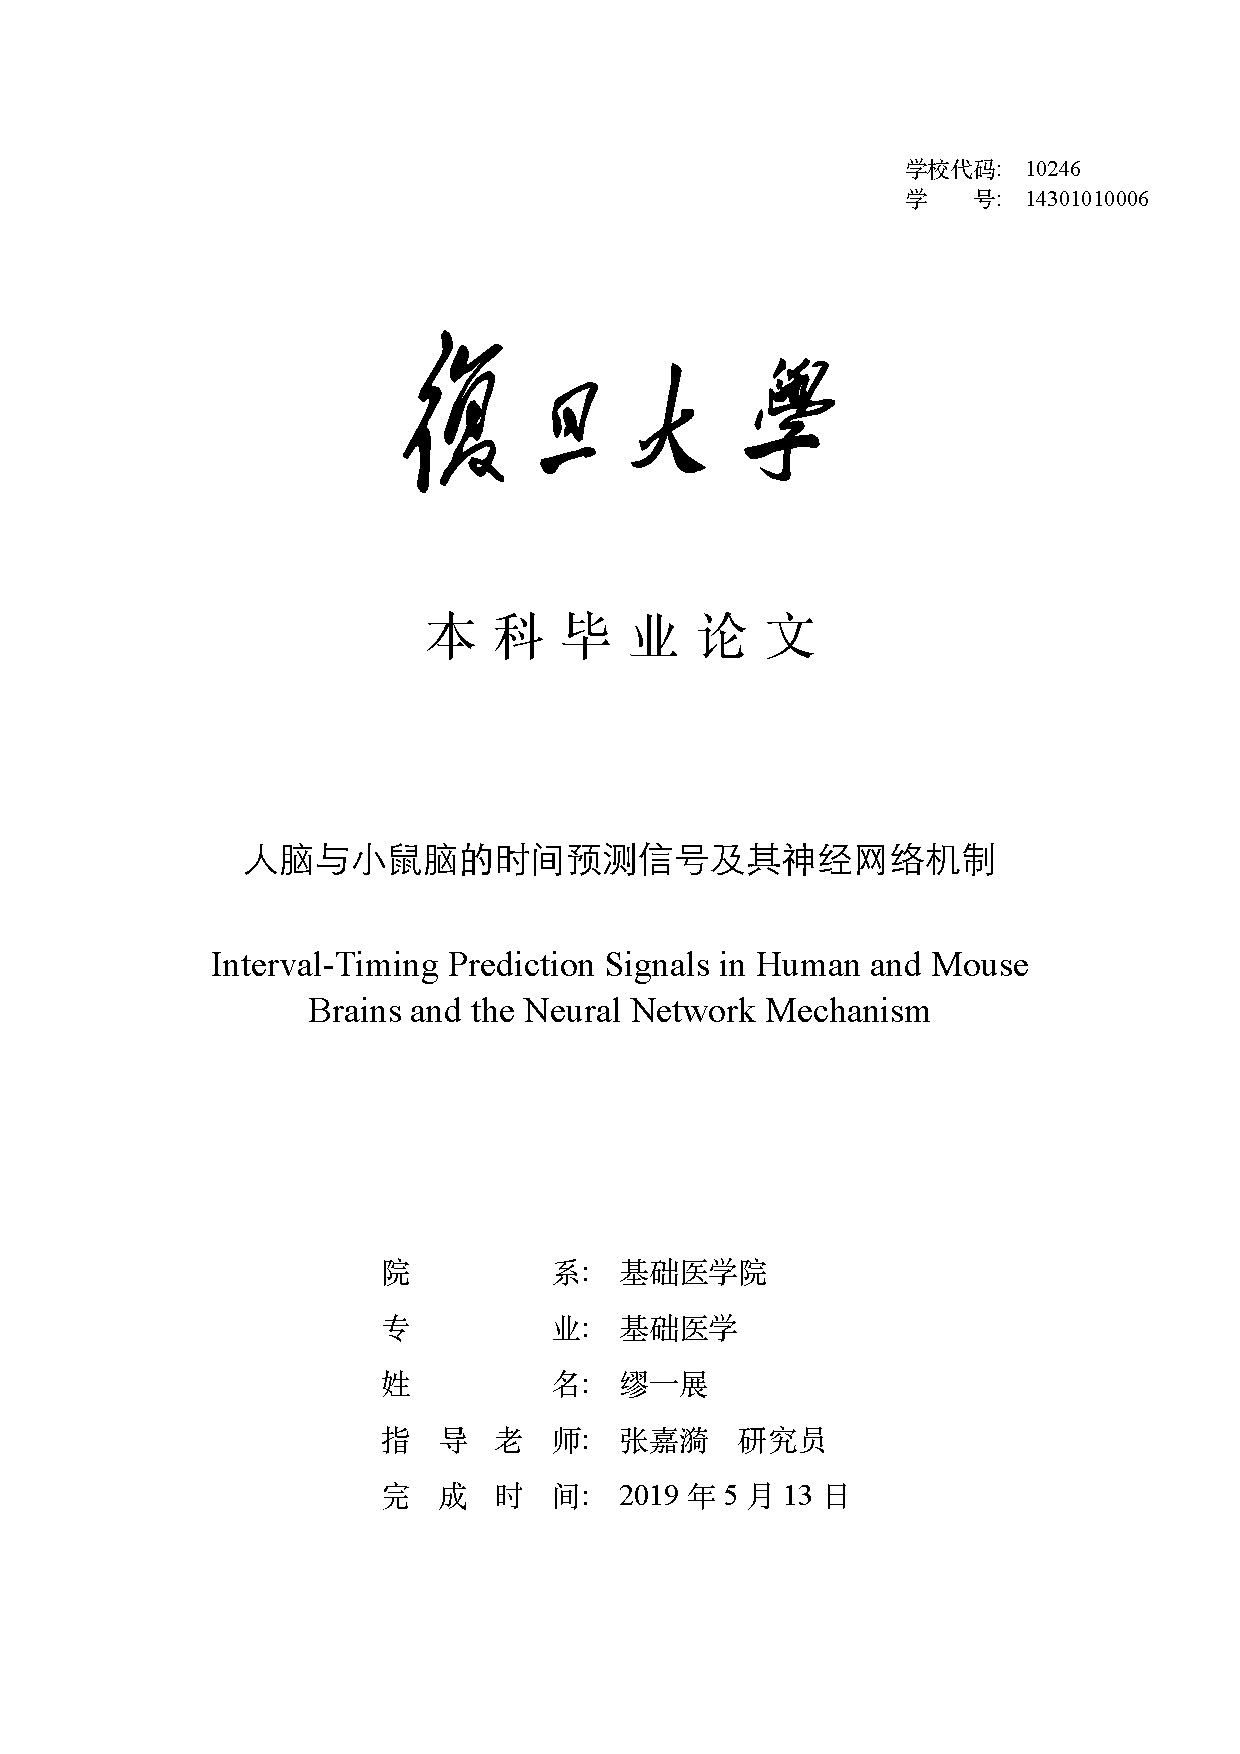
\includepdf{book-cover.pdf}
%\thispagestyle{empty}
% use \thispagestyle{} fancy, plain, empty to redefine Per/Page Header

% Outline
%% Computation
%% Algorithm
%% Implementation

%% title

\maketitle
%% abstract
\begin{abstract}
    这是一个小摘要。
\end{abstract}

% 引言
\section{引言}

% Timing and everyday life, why it is so important
%时间就好像空间一样,也是现实世界的重要组成部分。
%因而对于时间有好的掌控和理解,对于每个个体的学习、记忆、行为都至关重要。
时间和空间一样,也是现实世界的重要组成部分。而时间又同空间有本质上的差别,
时间不能像空间一样朝任意方向随意的移动,而只能朝一个方向以固定的速率前进。
因而生物体对时间感知无法像对空间一样具有主动的探索性或者多样性,
例如视觉中的方向选择性,海马里的place cell等。
另一方面,时间作为现实的一个维度,对视觉、听觉、触觉等等几乎所有的感觉和运动
甚至高级的皮层功能都是至关重要的,因而生物体神经系统对时间信息的编码应当
是普遍而广泛的。

% timing has different scales, it is the millisecond and second timing we are
% talking about.
不同于我们人造的时钟,生物体内对不同尺度的计时有着截然不同的生物学机制。
例如,微秒层次的计时,依赖于不同树突棘接受的动作电位到达树突的微小时间差异来实现;
生物体也主要用此来定位声音的来源\cite{moiseff1981neuronal}。
例如,以天计的生物钟,独立于动作电位依靠
转录、合成、降解的动态循环来实现;掌控着生物体的昼夜节律\cite{panda2002circadian}。
神经生物发展至今,已经发现和明确了许多机制,但对于毫秒和数秒层面计时的机制依然不是很明朗
\cite{buonomano2007biology,paton2018neural}。
而这个层次的计时也最为复杂和重要。它可以帮助生物体对即将到来的事件作出预判,
协助不同个体间的交流,让我们有能力创造出音乐,有能力用语言来交流等等。

% sensory timing and motor timing are different, but more and more articles
% talk about sensorimotor coupling and showing that they might come from the
% same neural circuit.
%对于毫秒和数秒层面计时,在过去常常分为感觉计时(sensory timing)和
%运动计时(motor timing)。感觉计时更关注于神经网络如何对外部刺激侦测
%并提取出时间序列,而运动时间更关注于如何主动的产生时间序列和预判的信号。
%随着研究的不断推进,人们发现在很多脑区和核团存在感觉运动的耦连(sensorimotor coupling)
对于时间感知和计时的理论模型大致可以分为两大类,即内在模型(intrisinc model)和
专用模型(dedicated model)\cite{ivry2008dedicated,paton2018neural}。
专用模型的主要观点在于大脑中存在特定的管理计时的区域,就好像视觉皮层主管视觉,
听觉皮层主管听觉一样,计时也存在特殊的计时相关皮层或核团。
而内在模型的主要观点在于计时是一切行为和功能所必需的一环,因而计时是广泛而普遍的,
不存在特定的计时脑区,而是分散于不同的皮层和核团,与不同的脑区所主要负责的功能相整合在一起。
%而随着各类研究的进行,有越来越多的证据表明内在模型可能更加符合实际情况。

% Timing has many unique properties, like weber's law and time warp.
% skip this part.

% for this review, we will talk about sensory timing, especially in V1.
% we will first review theoretical mechanisms for timing and some other
% empirical evidence. Finally, we will talk about some limitations of
% the current models and theories.
对于本综述,我们将主要回顾一下当前主流的对毫秒和数秒层面计时的理论机制和相关模型假说,
包括震荡模型(oscillation),缓坡模型(ramping model)以及动态系统(dynamic system);
其中,我们将着重探讨动态系统理论模型的细节。
最后,我们会进一步探讨一下当下这些机制和模型的主要优势和不足,以及未来的展望。


% 理论机制与实验依据
\section{理论机制与相关实验研究}
对计时机制的探究可以帮助我们更好的理解学习和记忆的原理,同时对于神经系统工作的
更加通用普适的理论模型的提出也至关重要。在这里,我们主要从细胞层面和环路层面两个角度来
回顾主要的理论模型和相关实验设计。

\subsection{细胞层面}
有越来越多的实验表明存在有神经元对特定的时间间隔或者频率有特异性。而这些特异性
产生的主要因素包括了各类受体,离子通道,以及short-term synaptic plasticity。

% 离子通道

% 突出可塑性

\subsection{环路层面}
神经元与其他细胞最大的区别在于其可兴奋性,由于其特殊的膜蛋白和离子通道,让神经元
能够利用膜电位的变化来传递信息。而在我们人类的大脑里有着%TODO
神经元,而它们形成的突触的数量则更加庞大。如此庞大的通信网络彼此密不可分,
又执行着%TODO

借助于多通道电极记录的技术,让我们可以对这个混沌系统有更近距离的观察。



$$ \frac{dX}{dt} = f(X) + U $$

%% this is the most interesting thing here.


% 计时与初级视皮层
\section{计时与初级视皮层}

初级视皮层(primary visual cortex, V1)再过去被认为只负责了简单的视觉信号的传递
和简单的处理,例如方向选择性等。而随着各类研究的深入,初级视皮层被发现能够
处理很多的高级功能。这也提示了大脑并不是一个严格分区分工的器官,而应该视作
一个整体;各个部分都互相连系并发挥着各自的影响。

Shuler实验室利用大鼠来对初级视皮层中的计时现象进行研究。他们首先利用训练大鼠
通过识别不同的视觉刺激来获得奖赏。而奖赏的大小与大鼠等待的时间存在一定的函数
关系。经过学习之后的大鼠可以在看到不同的刺激后,等待不同的时间再去触发奖赏。
利用多通道电生理记录,他们发现存在有神经元与计时显著相关。且神经元的活动
随着训练的增加而逐渐明显。

之后他们又利用药物干预的方法,证明了初级视皮层中的这些神经元与计时行为的好坏
存在因果关系。且学习新的计时涉及到了初级视皮层中的乙酰胆碱能相关的神经元或者突触。
随后他们又利用离体活体脑片膜片钳技术发现这些胆碱能主要来自L5/6的投射。最后他们
借助与光遗传的手段控制了从大鼠前额叶投射到初级视皮层的突触,证明了来自大鼠前额叶
的乙酰胆碱能神经元投射与初级视皮层形成新的计时行为存在因果关系。另一方面,
他们也表明大鼠的初级视皮层的活动与自主的计时行为存在相关性。


% 目前的局限所在与未来的发展
\section{小结与展望}

虽然大脑是我们人体中最为复杂和精细的器官,但它也是通过发育一点点成长而来;
从经济的角度而言,不同的感官不同的刺激不同的行为需要完全不同的算法和实现方法是
不经济的。而我们的大脑有着十分庞大的冗余量,不同的功能区也可以出现不同程度的相互替代,
这些都提示了大脑工作的背后可能存在着一个通用的算法,来支配着整个大脑的学习和活动。
另一方面,Saining Xie等人对神经网络的研究发现完全随机的神经网络有着和人为设计的
网络相似的正确率,有时甚至会比人为设计的网络有着更高的效率\cite{xie2019exploring}。
虽然这是一个纯理论的计算科学的研究,但也从它的角度为我们的神经科学提供了一些可能。

本综述简单的回顾了计时领域中常见的三大类理论模型: (1)振荡模型; (2)梯度模型; (3)动态系统。
每中模型都是对各自获得的实验结果的拟合和模拟。从过去的脑电和局部场电位变化获得的振荡模型,
到之后基于单通道电生理记录的梯度模型,和多通道电生理记录的动态系统。每种模型都有各自的优势
和可以用来解释的现象。而振荡模型和坡度模型所描述的现象可能只是动态系统的读出结果,
同时动态系统所描述的现象不仅可以用在计时中,也可以推广向不同的感觉和运动信息的处理。
因而相较而言,动态系统所描述的原理可能更接近于神经系统处理信息的方式方法。
但我们依然需要更多的实验和理论探究来解决大脑动态网络的出现原理和学习过程中大脑是如何
实现快速动态的调整等问题。



%\phantomsection
%\addcontentsline{toc}{chapter}{\bibname}
%\bibliographystyle{FDUbib}
%\bibliography{ThesisBib}

\end{document}
